\section{NUMERICAL EVALUATION OF SYSTEM DYNAMICS}

The obtained controller strategies in the previous section are applied to a finite-difference method (FDM) representation of the system model to evaluate the system dynamics. The system model is discretized in space and time, and the resulting system of ordinary differential equations is solved using the \texttt{`solve\_ivp'} function in Python's \texttt{`SciPy'} library \autocite{2020SciPy}, which employs the adaptive Runge-Kutta method of order 5(4), \texttt{`RK45'}. Each state of the system is discretized in space using 100 grid points. The \texttt{`RK45'} method automatically adjusts time steps to balance accuracy and computational efficiency, with the solution being evaluated at specific points as required. First, the unstable dynamics of the open-loop system is explored. Then two full-state feedback systems are compared with respect to number of eigenmodes used to obtain the optimal feedback gain. Finally, the performance of the proposed observer-based controller is evaluated and the state reconstruction error dynamics are analyzed.

\subsection{FDM representation of the open-loop system}

The open-loop system dynamics are first explored using a finite-difference method (FDM) representation. The system model is discretized in space and time, and the resulting system of ordinary differential equations is solved using the \texttt{solve\_ivp} function in Python. The 3D plot in Figure \ref{fig:3D_x1_openloop} illustrates the unstable dynamics of the open-loop system over time.

\begin{figure}[H]
    \centering
    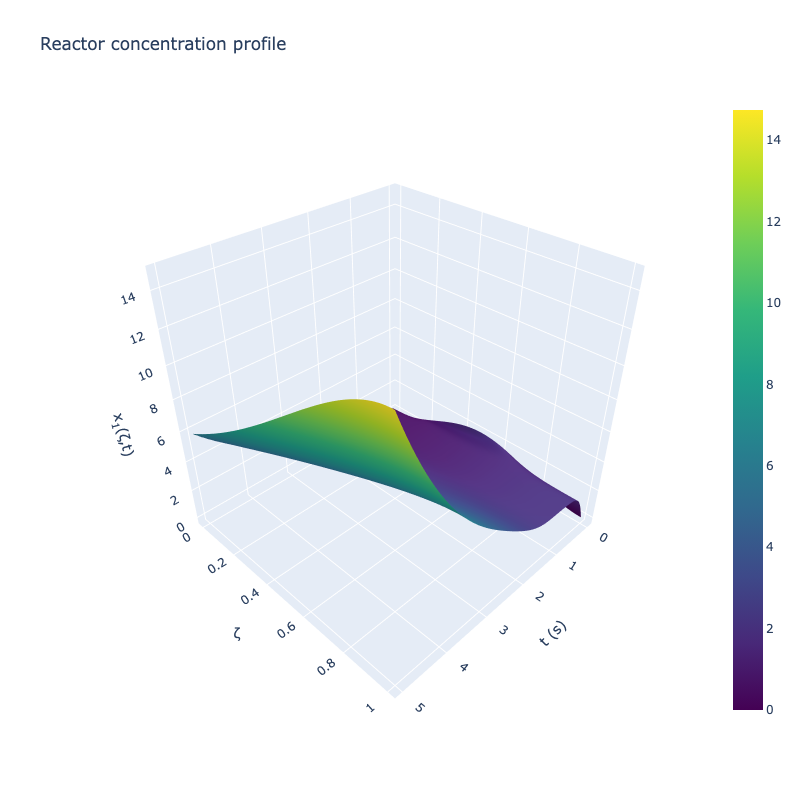
\includegraphics[width=0.8\textwidth]{Figures/3D_x1_openloop.png}
    \caption{3D plot of the open-loop system}
    \label{fig:3D_x1_openloop}
\end{figure}

\subsection{Full-state feedback regulator FDM representation}

Next, the full-state feedback regulator is evaluated using an FDM representation. Two configurations are compared: one with $N=3$ eigenmodes and another with $N=7$ eigenmodes. Figures \ref{fig:3D_x1_k3} and \ref{fig:3D_x1_k7} show the 3D plots of the system dynamics for these configurations. The 2D plot in Figure \ref{fig:2D_xt_k7} provides a detailed view of the state trajectories for the $N=7$ configuration.

\begin{figure}[H]
    \centering
    \begin{subfigure}[b]{0.45\textwidth}
        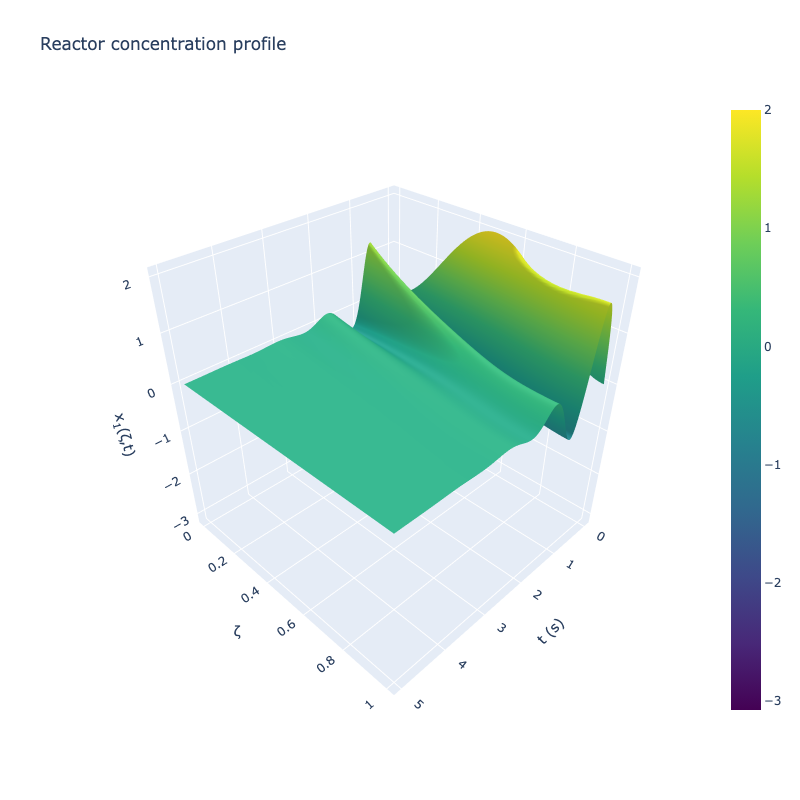
\includegraphics[width=\textwidth]{Figures/3D_x1_k3.png}
        \caption{Full-state feedback regulator with $N=3$}
        \label{fig:3D_x1_k3}
    \end{subfigure}
    \hfill
    \begin{subfigure}[b]{0.45\textwidth}
        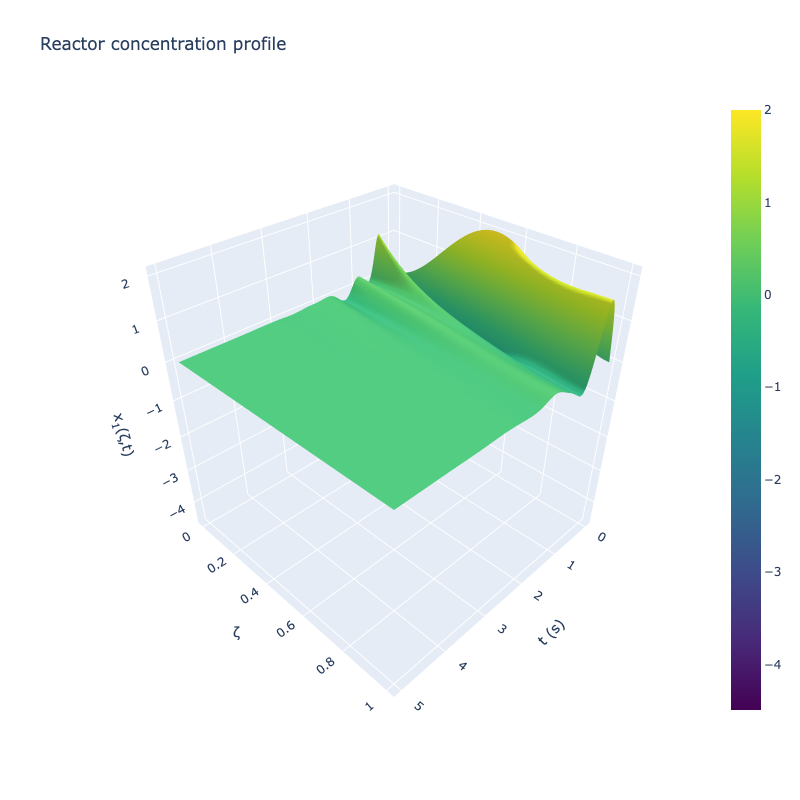
\includegraphics[width=\textwidth]{Figures/3D_x1_k7.png}
        \caption{Full-state feedback regulator with $N=7$}
        \label{fig:3D_x1_k7}
    \end{subfigure}
    \caption{FDM representation of the full-state feedback regulator}
    \label{fig:full_state_feedback}
\end{figure}

\begin{figure}[H]
    \centering
    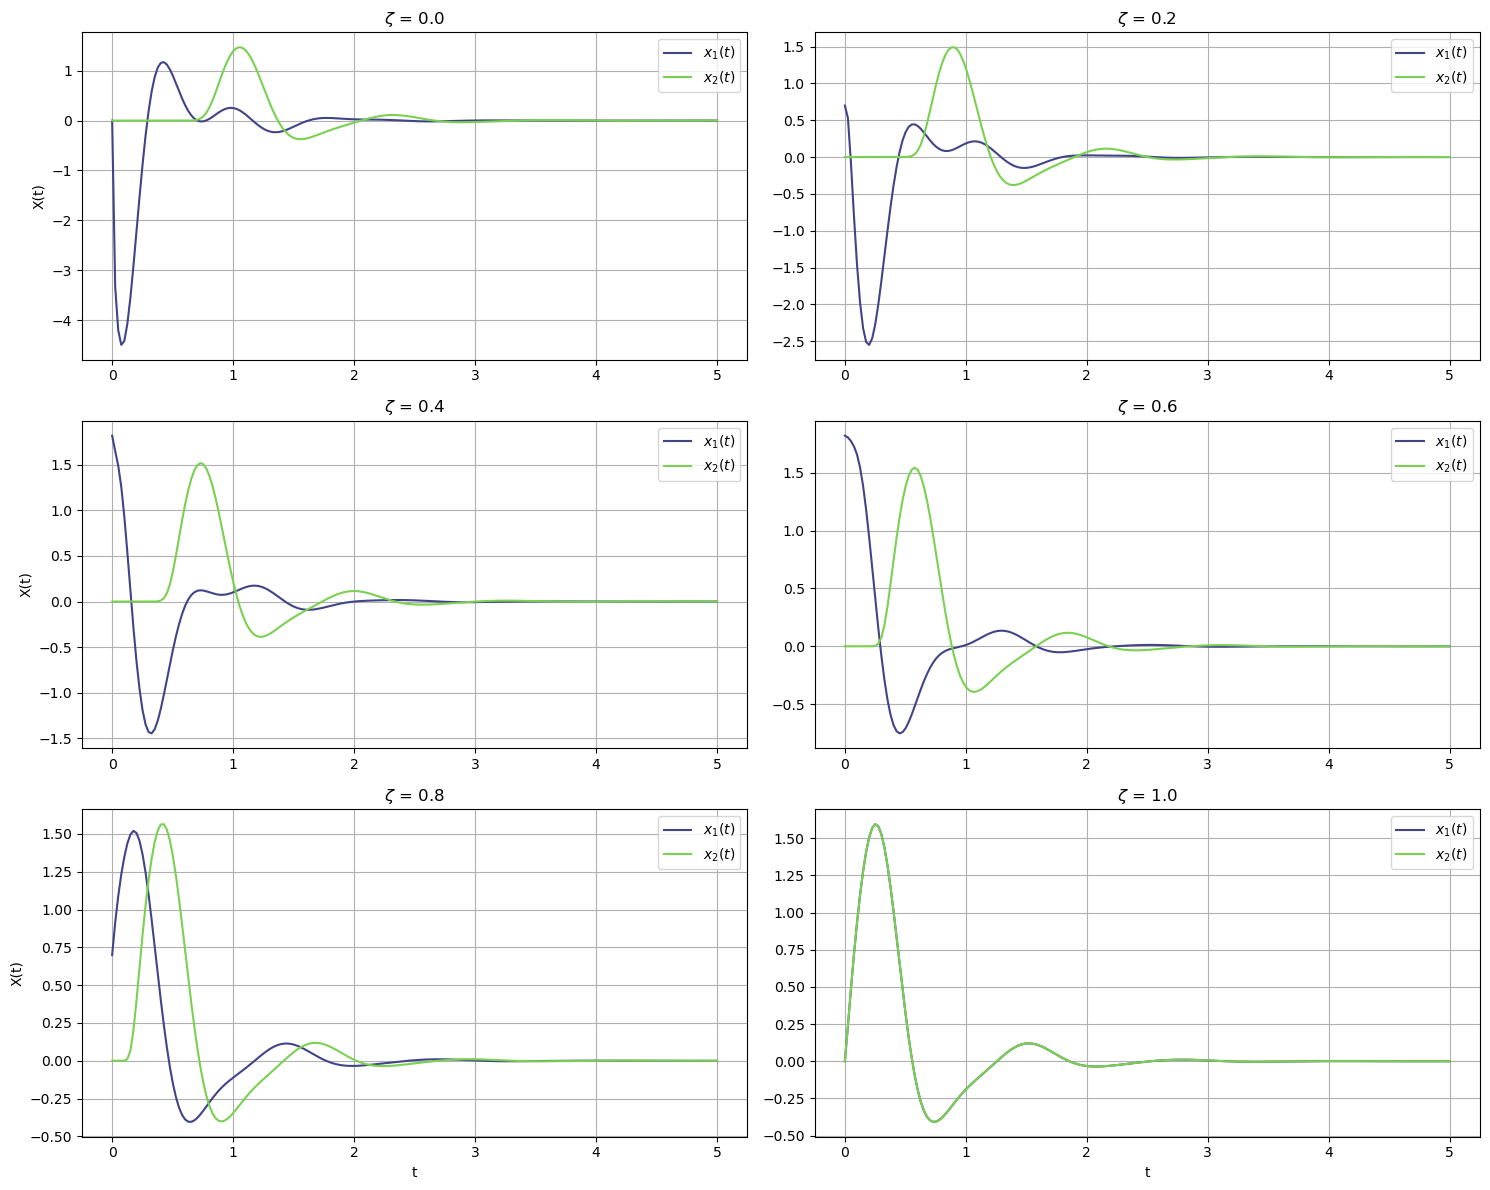
\includegraphics[width=0.8\textwidth]{Figures/2D_xt_k7.png}
    \caption{2D plot of the full-state feedback regulator with $N=7$}
    \label{fig:2D_xt_k7}
\end{figure}

\subsection{Observer-based regulator FDM representation}

Finally, the observer-based regulator is evaluated using an FDM representation. The system model is discretized in space and time, and the resulting system of ordinary differential equations is solved using the \texttt{solve\_ivp} function in Python. Figures \ref{fig:3D_x1_L_k7} and \ref{fig:2D_xt_L_k7} show the 3D and 2D plots of the observer-based regulator, respectively. The error dynamics of the observer-based regulator are illustrated in Figures \ref{fig:3D_e1_L_k7} and \ref{fig:2D_et_L_k7}, providing insights into the state reconstruction error over time.

\begin{figure}[H]
    \centering
    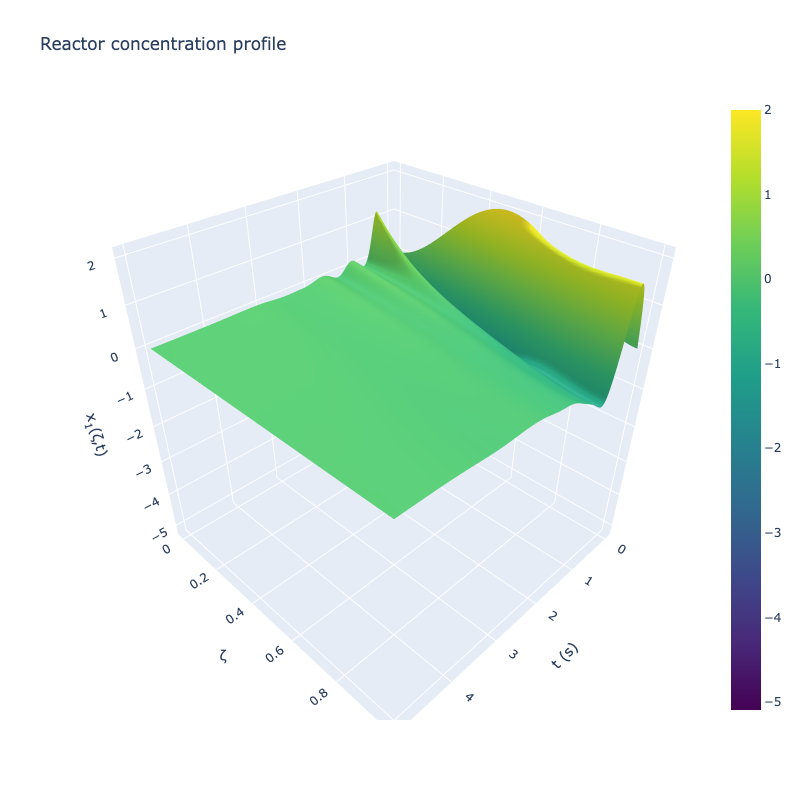
\includegraphics[width=0.8\textwidth]{Figures/3D_x1_L_k7.png}
    \caption{3D plot of the observer-based regulator}
    \label{fig:3D_x1_L_k7}
\end{figure}

\begin{figure}[H]
    \centering
    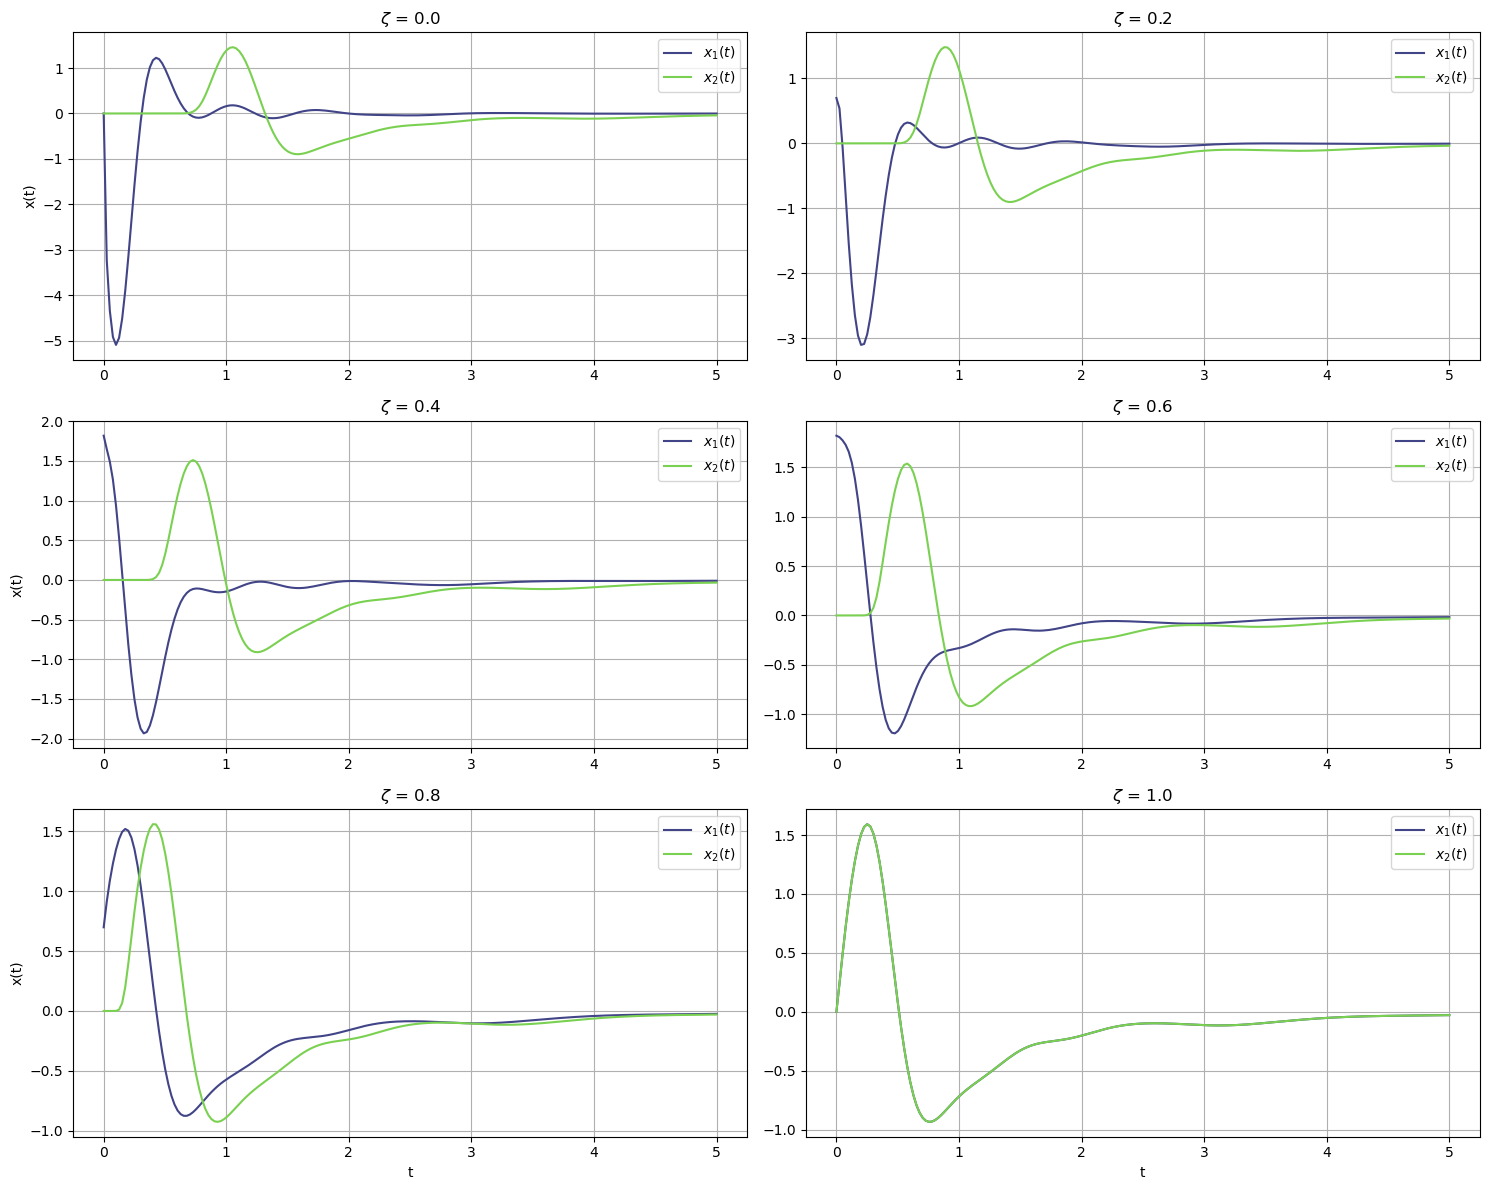
\includegraphics[width=0.8\textwidth]{Figures/2D_xt_L_k7.png}
    \caption{2D plot of the observer-based regulator}
    \label{fig:2D_xt_L_k7}
\end{figure}

\begin{figure}[H]
    \centering
    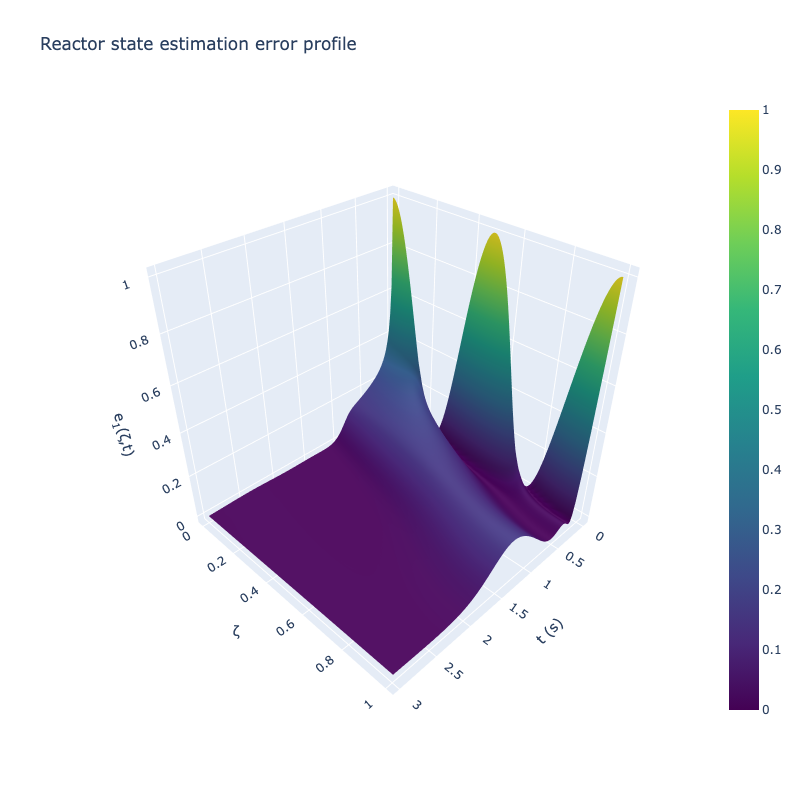
\includegraphics[width=0.8\textwidth]{Figures/3D_e1_L_k7.png}
    \caption{3D plot of the error dynamics of the observer-based regulator}
    \label{fig:3D_e1_L_k7}
\end{figure}

\begin{figure}[H]
    \centering
    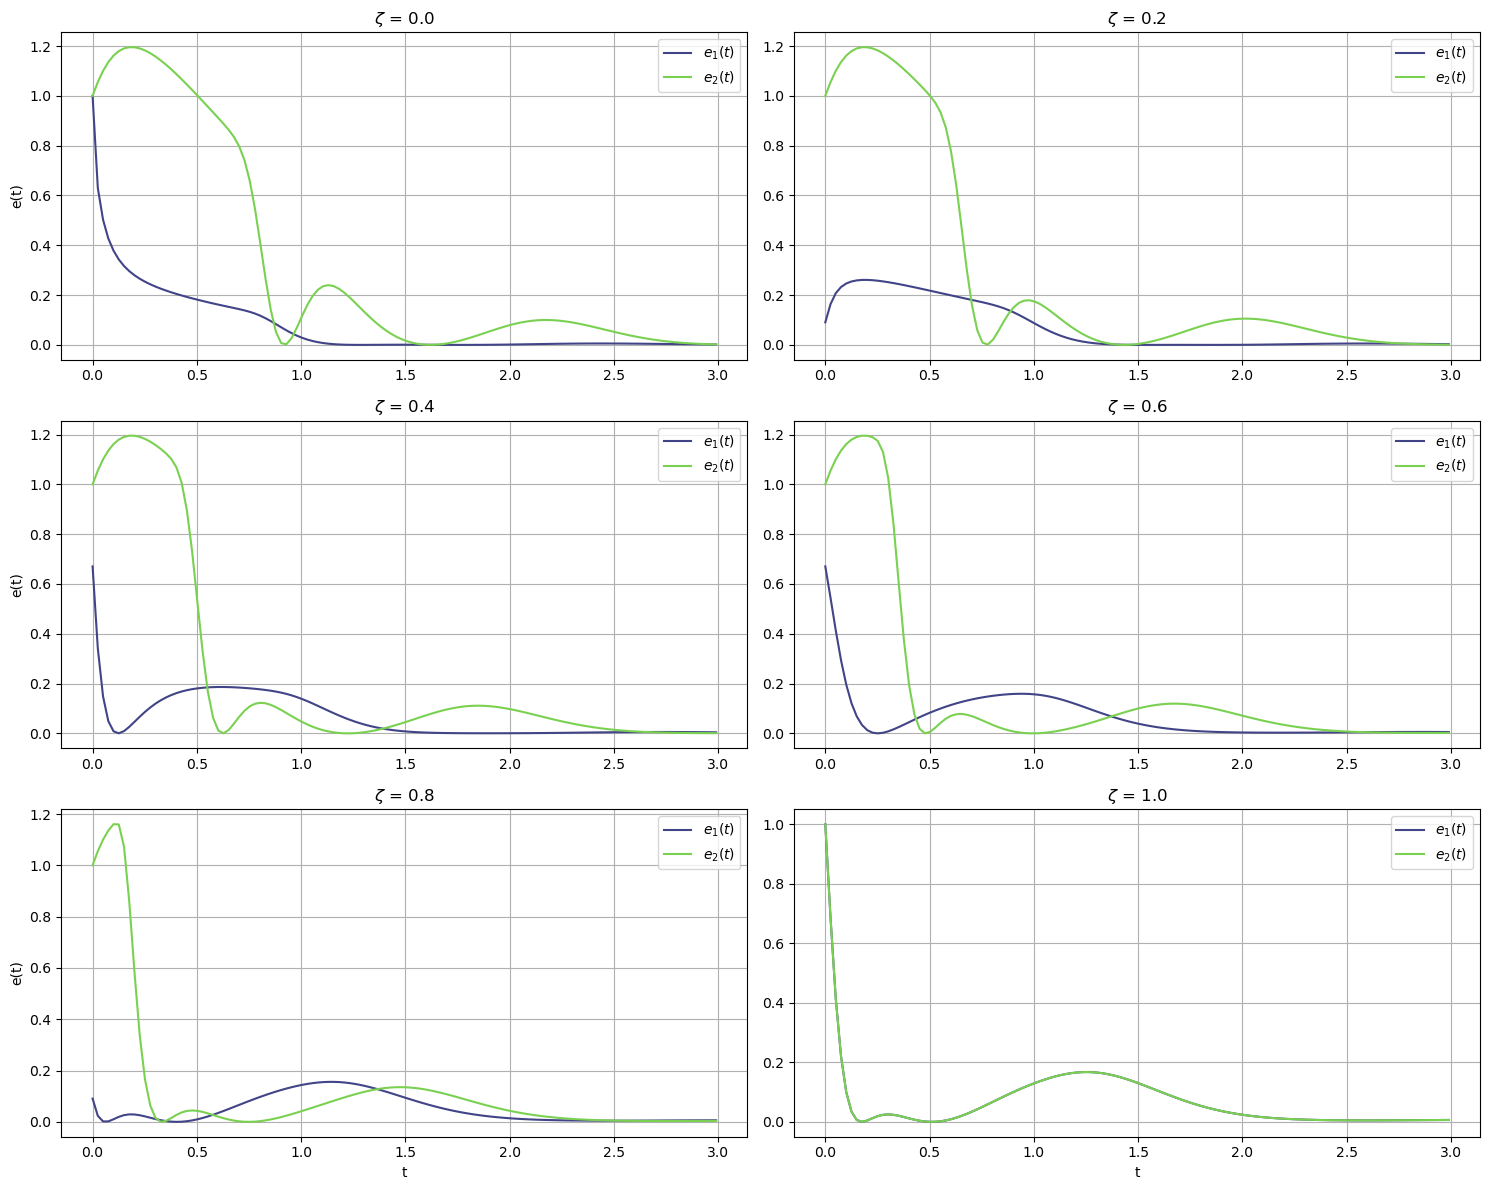
\includegraphics[width=0.8\textwidth]{Figures/2D_et_L_k7.png}
    \caption{2D plot of the error dynamics of the observer-based regulator}
    \label{fig:2D_et_L_k7}
\end{figure}